\chapter{Few-Shot Learning}\label{chap:fsl}
A good machine learning model often requires training with a large number of samples. Humans, on the contrary, learn new concepts and skills much faster and more efficiently. Children who have only seen cats and birds a few times can quickly tell them apart. People who know how to ride a bike are likely to discover how to ride a motorcycle quickly with little or even no demonstration. Is it possible to design a machine learning model with similar properties - learning new concepts and skills fast with a few training examples? That is essentially what few-shot learning is designed to solve.

Despite notable advances in the field of artificial intelligence, two essential aspects of human conceptual intelligence have consistently eluded machine learning and artificial intelligence (AI) systems. 
First, for most interesting kinds of natural and man-made categories of entities, humans can learn a new concept from just one or a few handful examples, whereas many AI models would require several thousands of examples to perform satisfactorily. 
Second, people learn far richer representations than machines do, even for seemingly simple concepts, and use them for a wide variety of tasks such as creating new entities based on the exemplars, classifying objects into parts, grasping between concepts and parts, and creating new abstract categories (concepts) by combining existing ideas and concepts.
In contrast to this, the best machine learning models and neural networks cannot perform these additional functions using their specialised learnt representations. 
The challenge arises when we wish for AI models to learn new concepts and representations from few examples and ensure that these representations are abstract and flexible.

\section{Formalising the Few-Shot Learning Problem}\label{sec:formalising-fsl}

In a few-shot setting, the model aims to generalise well and quickly enough on a variety of new and potentially unseen tasks after being trained for optimal performance on various learning tasks.
Each task is associated with a dataset $\mathcal{D}$, containing both inputs and true labels. 
The model parameters of an optimal generalisable model are defined as follows:
\begin{equation}
    \symbfit{\theta}^\star = \arg\min_{\symbfit \theta} \mathbb{E}_{\mathcal{D}\sim p(\mathcal{D})} [\mathcal{L}_{\symbfit \theta}(\mathcal{D})]
\end{equation}

First, we look at how \(\mathcal{D}\) is structured in a standard supervised few shot setting. 
Consider a labelled dataset $\mathcal{D} = \left\{(\symbfit{x}_i, y_i)\, |\, i \in [1,N^{'}] \right\}$ of images $\symbfit{x}_i$ and class labels $y_i$. 
This dataset $\mathcal{D}$ is divided into three disjoint subsets: $\left\{\mathcal{D}^\textup{tr}\, \cup\, \mathcal{D}^\textup{val}\, \cup\, \mathcal{D}^\textup{test}\right\} \in \mathcal{D}$, respectively, referring to the training, validation, and test subsets. The validation dataset $\mathcal{D}^\textup{val}$ is used for model selection and the testing dataset $\mathcal{D}^\textup{test}$ for final evaluation. The episodic training is done on a set of tasks $\mathcal{T}_i \sim p(\mathcal{T})$. The tasks are constructed by drawing $K$ random samples from $N$ different classes, which we denote as an ($N$-way, $K$-shot) task. 
Specifically, each task $\mathcal{T}_i$ is made up of a set $\textit{support}$ and a $\textit{query}$ set. The support set $\mathcal{S}$ contains $K$ samples per class and the query set $\mathcal{Q}$ contains $Q$ samples per class. For a given task, the $NK$ support and $NQ$ query images are mutually exclusive to evaluate the generalisation performance of the model.
In most training routines, tasks are sampled randomly from the distribution of tasks according to the $N$-way, $K$-shot setting, and then the model parameters are updated via backpropagation after each task. This comprises of one episode. 

\begin{figure}[ht]
    \centering
    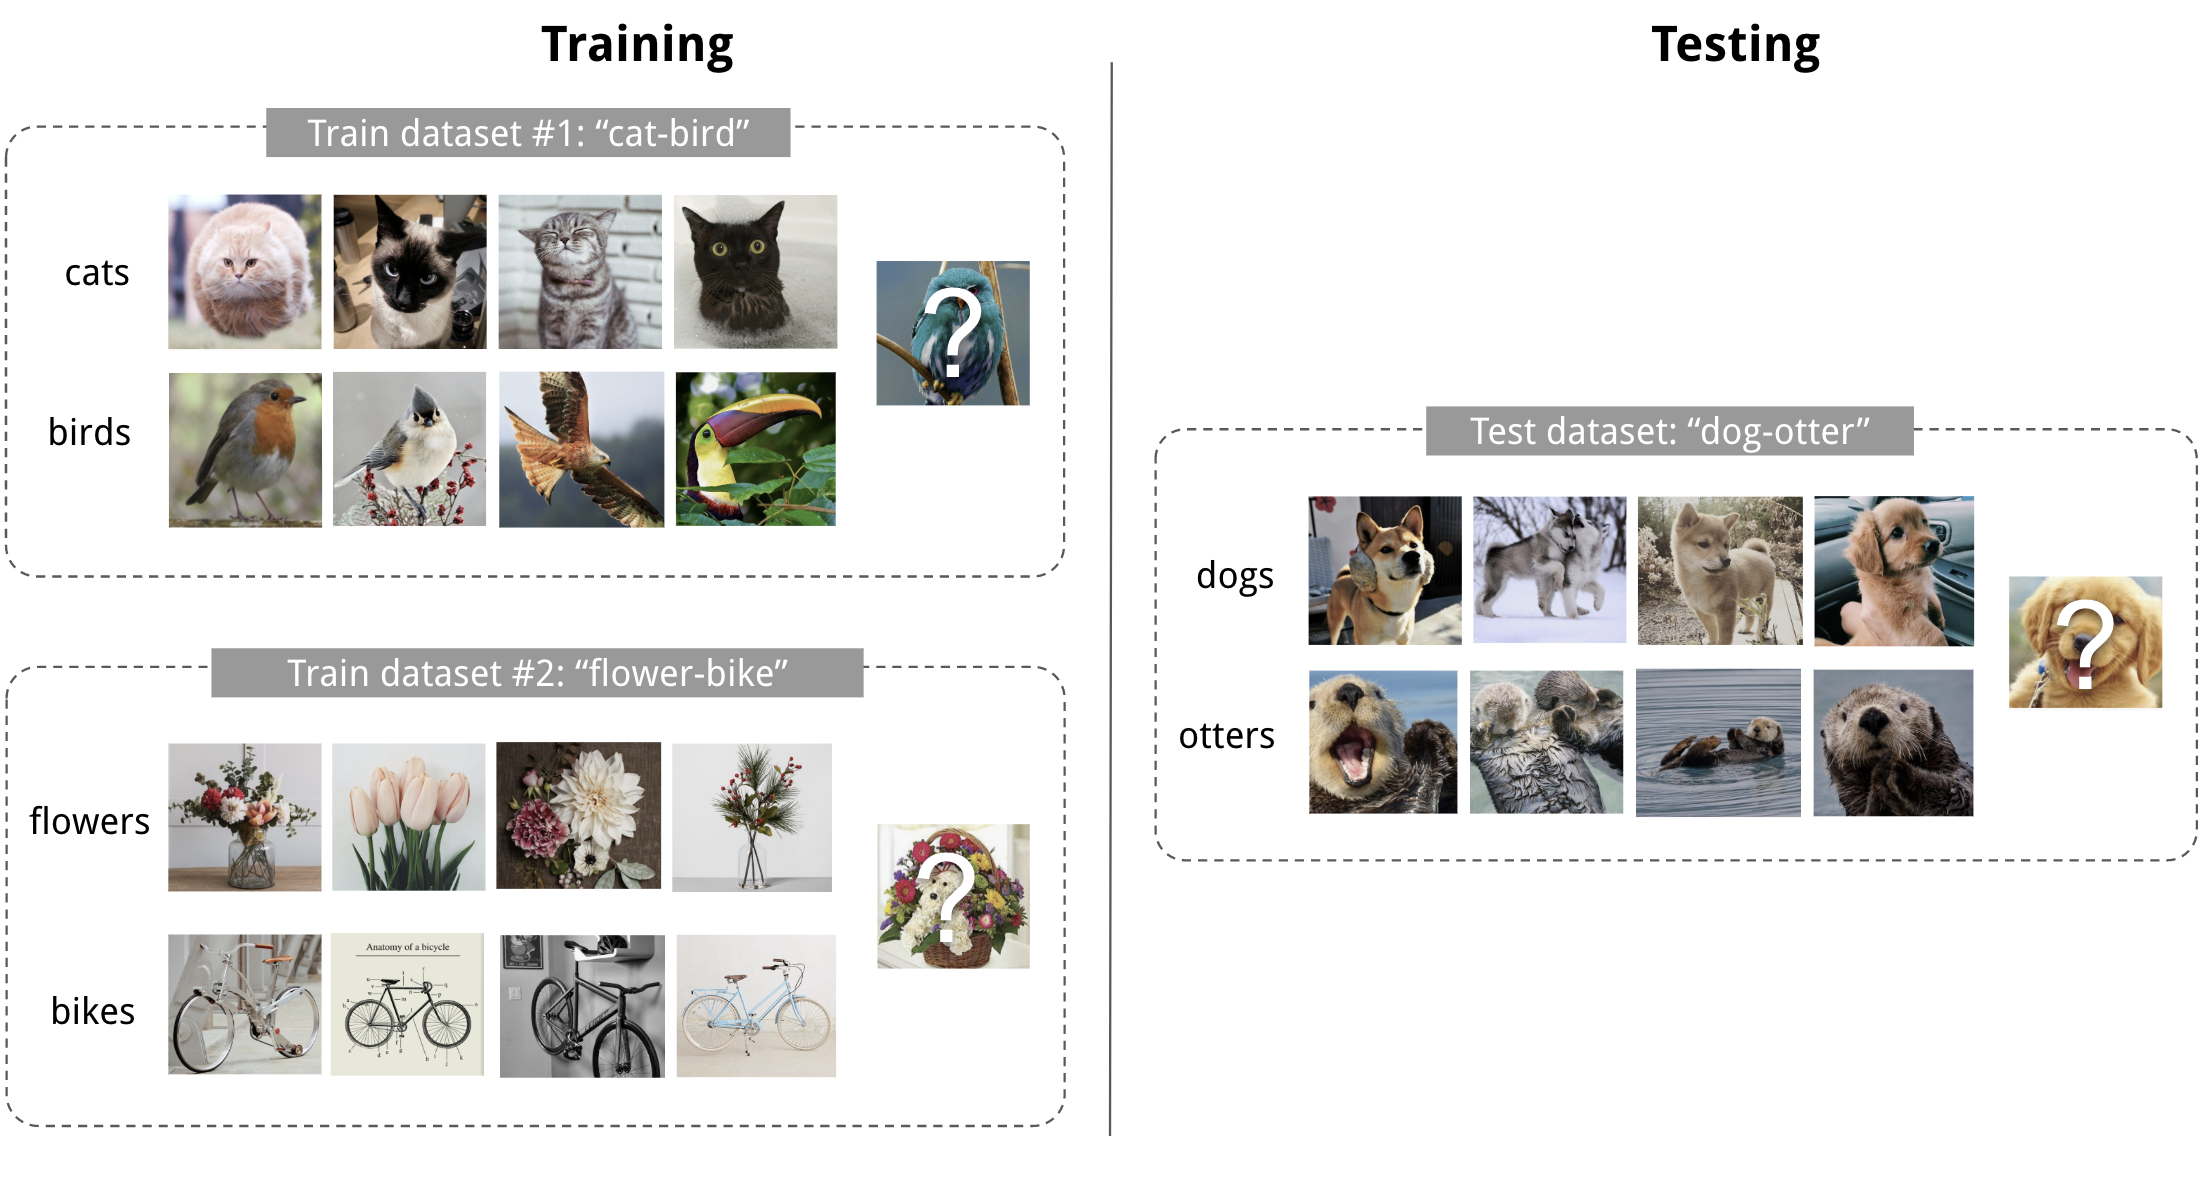
\includegraphics[scale=0.4]{chapters/assets/fsl/few-shot-classification.png}
    \caption{An example of 4-shot 2-class image classification.}
    \label{fig:fsl-tasks}
\end{figure}



%Let us denote the training data of size $D$ as $\mathcal{D}_{\textup{tr}} = \{({\bm x}_i, y_i)\}_{i = 1}^{D}$ with $({\bm x}_i, y_i)$ representing an image and its class label, respectively. In the pre-training phase, we take $L$ random samples from $\mathcal{D}_{\textup{tr}}$ and augment each sample $A$ times by randomly sampling augmentation functions $\zeta^a(.), \forall a \in [A]$ from the set $\mathcal{A}$. This results in a mini-batch of size $B = (A + 1)L$ total samples. Note that in the unsupervised setting we have no access to the data labels in the pre-training phase. Next, we fine-tune our model episodically \cite{Vinyals2016MatchingLearning} on a set of randomly sampled tasks $\mathcal{T}_i$ drawn from the test dataset $\mathcal{D}_{\textup{tst}} = \{({\bm x}_i, y_i)\}_{i = 1}^{D^\prime}$ of size $D^\prime$. The tasks $\mathcal{T}_i$ are constructed by drawing $K$ labeled and $Q$ unlabeled random samples from $N$ different classes, which is called an ($N$-way, $K$-shot) task, and denoted by $(N, K)$. The $NK$ labeled samples make up the support set $\mathcal{S}$, from which the model learns, and the other $NQ$ unlabeled samples make up the query set $\mathcal{Q}$, on which the model is evaluated
